%%=============================================================================
%% Basisfunctionaliteiten
%%=============================================================================

\chapter{Basisfunctionaliteiten}%
\label{ch:basisfunctionaliteiten}

In dit hoofdstuk gaan we de basisfunctionaliteiten van native en cross-platform vergelijken. 
Met deze resultaten kunnen we dan een gepaste conclusie vormen.

\section{Native}
\subsubsection{Wat hebben we nodig}
Normaal gezien zullen we voor de functionaliteiten altijd een of andere library of API gebruiken. Enkel bij de navigatie is dit niet nodig. 
Voor de navigatie zullen we gebruik maken van een startproject dat Android Studio aanbied, hierin zit de navigatie al geïmplementeerd 
\ref{par:basisfunctionaliteiten}. Voor het laadscherm dat getoond wordt bij het opstarten van de applicatie gaan we wel een externe API gebruiken. 
Deze is de SplashScreen API \url{https://developer.android.com/develop/ui/views/launch/splash-screen#getting-started}.

\subsubsection{Uitvoering}

Voor de navigatie was het voldoende om het nieuw project aan te maken. 
Hierbij zit de navigatie al geïmplemnteerd.

\paragraph{1. Gradle instellingen aanpassen}
Om de SplashScreen API te gebruiken, moeten we deze aan onze dependacies toevoegen. Dit doen we in
het \textbf{build.gradle(module)} bestand.
\begin{minted}{kotlin}
dependencies {
    // andere dependacies
    implementation("androidx.core:core-splashscreen:1.0.0")
}
\end{minted}

\paragraph{2. SplashScreen instellen}
Na het toevoegen van de dependancy kunnen we het laadscherm customizen op basis van onze wensen. 
Hiervoor maken we een nieuw \textbf{splash.xml} bestand in de \textbf{res/values} map. In dit 
bestand kunnen we dan het laadscherm customizen. Ook voegen we hier een icon toe dat zal worden
getoond tijdens het laden. Dit icoon moet in de \textbf{res/drawable} map worden geplaatst.
\begin{minted}{xml}
<?xml version="1.0" encoding="utf-8"?>
<resources>
    <style name="Theme.MyApp.MySplash" parent="Theme.SplashScreen">
        <item name="windowSplashScreenBackground">@color/black</item>
        <item name="windowSplashScreenAnimatedIcon">@drawable/bank_svgrepo_com</item>
        <item name="postSplashScreenTheme">@style/Theme.Basis</item>
    </style>
</resources>
\end{minted}

\paragraph{3. Applicatie maken}
Dankzij deze informatie kunnen we een applicatie opzetten dat een laadscherm toont dat zal verdwijnen 
van zodra de applicatie zijn eerste frame tekent. Daarna is er een navigatiebar te zien onderaan die ervoor zorgt dat 
we kunnen navigeren tussen de verschillende schermen.
\begin{figure}[H]
    \centering
    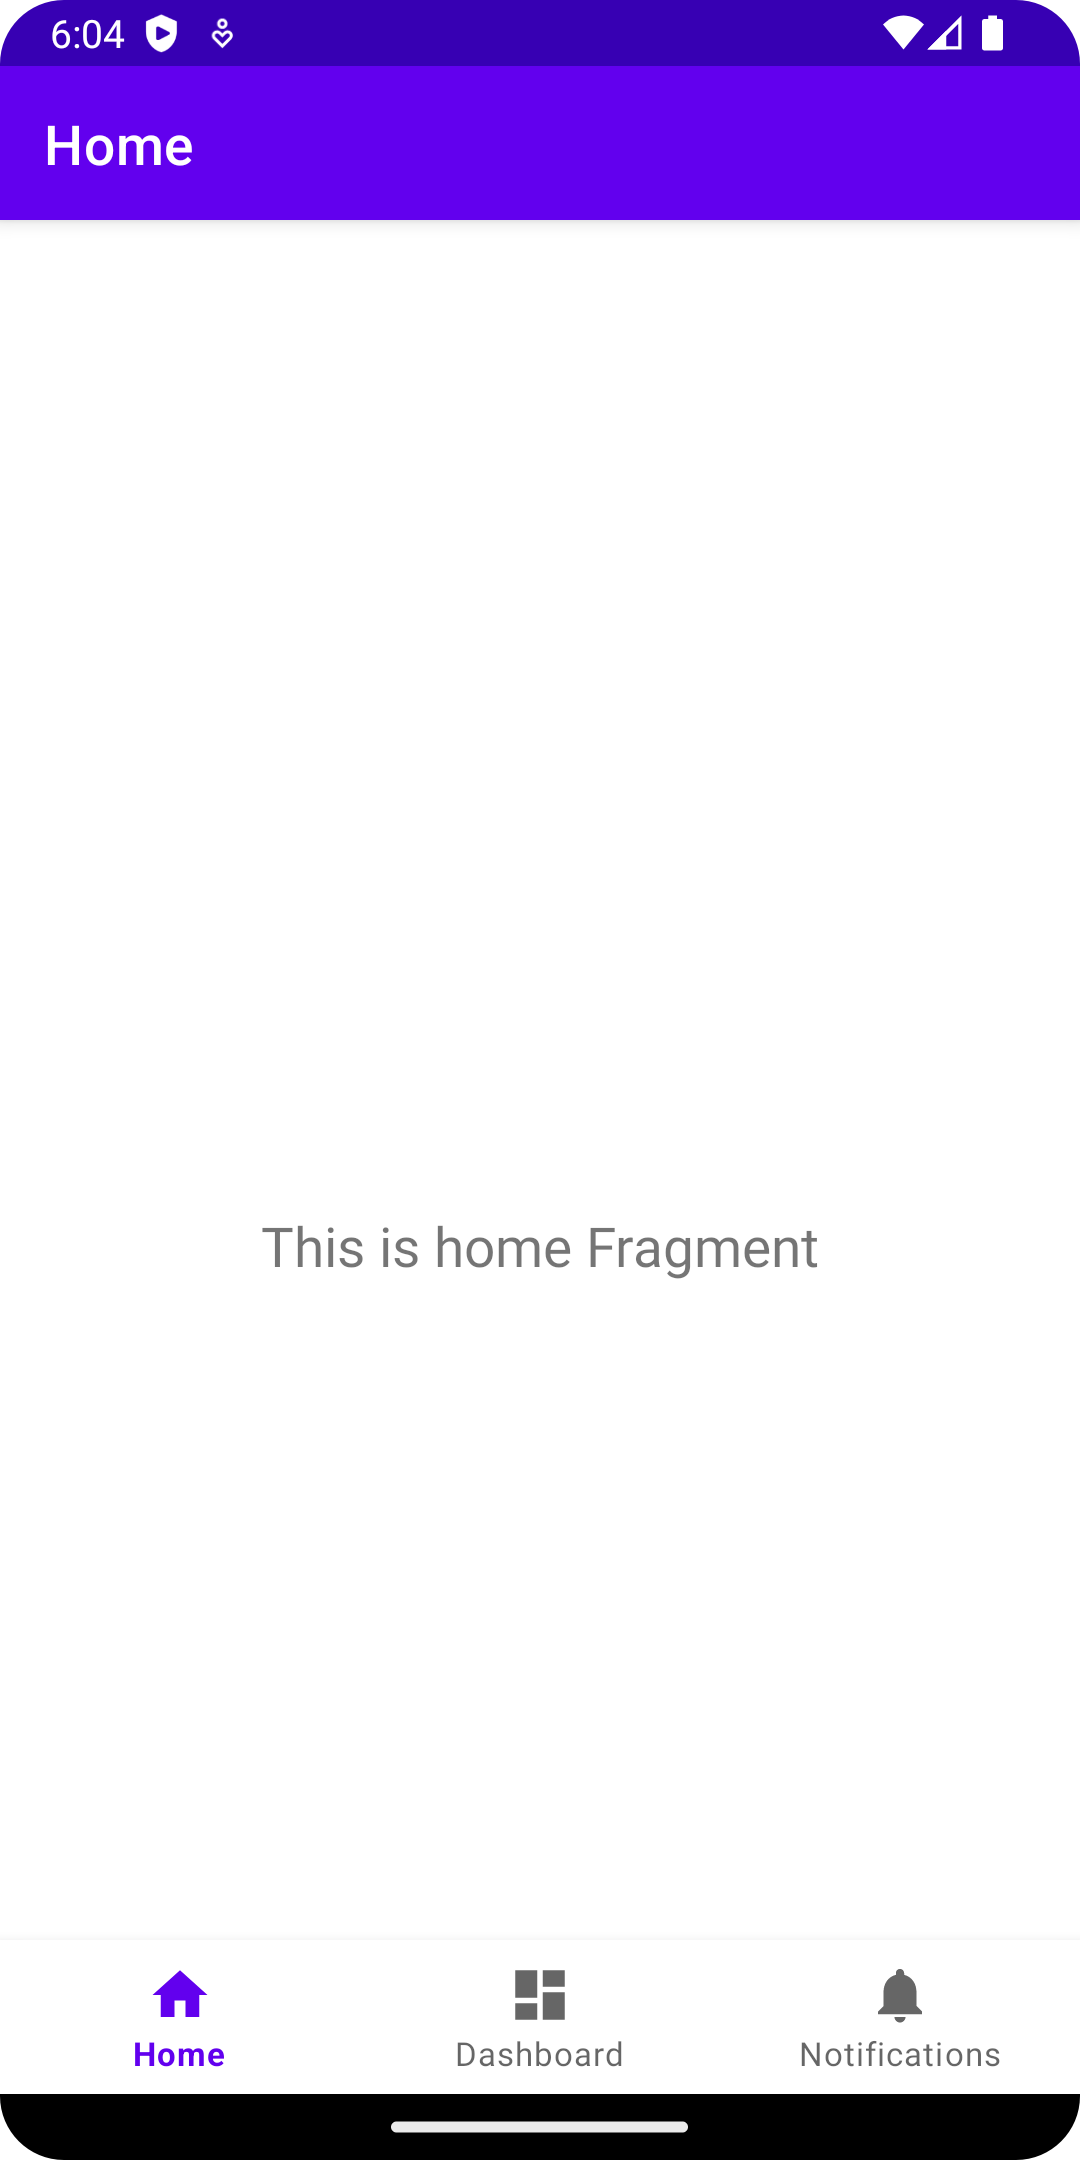
\includegraphics[height=0.5\textheight]{basis_layoutnative.png}
    \caption{Layout van applicatie voor de basisfunctionaliteiten bij Android.}
\end{figure}


\subsubsection{Ontwikkeltijd}

Dankzij het startproject dat Android Studio aanbiedt, is het mogelijk om snel een applicatie op te zetten 
die gebruik maakt van de navigatiecomponent. Daarnaast kan het laadscherm ook snel geïmplementeerd worden. 
Er moet enkel al een icon aanwezig zijn om te tonen. Om de volledige applicatie aan te maken inclusief opzoekwerk
en het aanmaken van de icoon
is er 1 uur en 15 minuten gespendeerd.



\subsubsection{Performantie}

\paragraph{Tijdsduur}

\paragraph{CPU \& geheugen}

\subsubsection{Schaalbaarheid}

\paragraph{Complexiteit}
De navigatie is niet complex om op te zetten aangezien een startproject kan worden gebruikt.
Daarnaast is het ook niet complex om schermen toe te voegen of aan te passen.
Dankzij de Splashscreen API is ook het laadscherm niet complex om op te zetten. 
Het enige dat nodig is, is een icoon om te tonen.

\paragraph{Herbruikbaarheid}
De navigatie kan zoals hierboven vermeld gemakkelijk hergebruikt worden om extra schermen 
toe te voegen en is dus zeer schaalbaar.
Het is ook gemakkelijk om de bestaande schermen te hergebruiken in andere applicaties. 
Bij het laadscherm is er geen sprake van opschaling. Dit is enkel nodig bij het opstarten 
van de applicatie en zal dus maar één keer geïmplementeerd moeten worden.



\section{Cross-platform}
\subsubsection{Wat hebben we nodig}


\subsubsection{Uitvoering}

\paragraph{1. Library toevoegen}
Om de navigatie en het laadscherm te kunnen gebruiken, moeten de juiste libraries aan 
de root van het project worden toegevoegd. Deze worden toegevoegd met volgende commando's:
\begin{minted}{bash}
npm install @react-navigation/native
npm install react-native-screens
npm install react-native-safe-area-context
npm install @react-navigation/bottom-tabs
\end{minted}

\paragraph{2. onCreate methode toevoegen}
Om de navigatie te gebruiken, moet een \textbf{onCreate} methode worden toegevoegd aan het
\textit{android/app/src/main/java/com/project/MainActivity.java} bestand.
\begin{minted}{java}
import android.os.Bundle;
// ...
public class MainActivity extends ReactActivity {
  // ...
  @Override
  protected void onCreate(Bundle savedInstanceState) {
    super.onCreate(null);
  }
  // ...
}
\end{minted}

\paragraph{3. Dependencies toevoegen}
Om het laadscherm te gebruiken, moeten de juiste dependencies worden toegevoegd aan het
\textit{android/app/build.gradle} bestand.
\begin{minted}{java}
dependencies {
  // Andere dependencies
  implementation("androidx.core:core-splashscreen:1.0.0")
}
\end{minted}

\paragraph{4. Laadscherm toevoegen}
Om een eerste laadscherm te genereren, kan volgend commando worden gebruikt:
\begin{minted}{bash}
npx react-native generate-bootsplash path/to/icon.png
    --background-color "#000000" 
    --logo-width=100 
    --assets-path=assets 
    --flavor=main 
    --platforms=android,ios
\end{minted}
Daarna moet er een stijl worden aangemaakt om het laadschem te tonen. Dit gebeurt in 
het \textit{android/app/src/main/res/values/styles.xml} bestand.
\begin{minted}{xml}
<style name="BootTheme" parent="Theme.SplashScreen">
    <item name="windowSplashScreenBackground">@color/bootsplash_background</item>
    <item name="windowSplashScreenAnimatedIcon">@mipmap/bootsplash_logo</item>
    <item name="postSplashScreenTheme">@style/AppTheme</item>
</style>
\end{minted}
Om bij het opstarten van de applicatie het laadscherm eerst te tonen, moet de volgende 
lijn in het \textit{android/app/src/main/AndroidManifest.xml} bestand worden aangepast.
\begin{minted}{xml}
<application
  android:name=".MainApplication"
  android:label="@string/app_name"
  android:icon="@mipmap/ic_launcher"
  android:roundIcon="@mipmap/ic_launcher_round"
  android:allowBackup="false"
  android:theme="@style/BootTheme"> <!-- Verander deze lijn -->
  <!-- ... -->
</application>
\end{minted}
Tot slot kan het laadscherm geïnitialiseerd worden door volgende regels toe te voegen aan het
\textit{android/app/src/main/java/com/project/MainApplication.java} bestand.
\begin{minted}{java}
import com.zoontek.rnbootsplash.RNBootSplash;

public class MainApplication extends Application implements ReactApplication {
  // ...
  @Override
  public void onCreate(Bundle savedInstanceState) {
    RNBootSplash.init(this); // Voeg deze lijn toe
    super.onCreate(savedInstanceState);
  }
  // ...
}
\end{minted}

\paragraph{5. Navigatie toevoegen}
Om de navigatie te gebruiken, moeten alle componenten in een 
\textbf{NavigationContainer} component worden gestoken. Dit wordt gedaan door volgende regels toe te voegen
aan het \textit{App.tsx} bestand:
\begin{minted}{javascript}
import { NavigationContainer } from '@react-navigation/native';

export default function App() {
  return (
    <NavigationContainer>
      {/* ... */}
    </NavigationContainer>
  );
}
\end{minted}

\paragraph{6. Bottom Tab navigatie toevoegen}
Om de bottom tab navigatie te gebruiken, moet een \textbf{createBottomTabNavigator}
functie worden aangemaakt. Dit wordt gedaan door de volgende regels toe te voegen aan het \textit{App.tsx} bestand:
\begin{minted}{javascript}
import { createBottomTabNavigator } from '@react-navigation/bottom-tabs';

const Tab = createBottomTabNavigator();

export default function App() {
  return (
    <NavigationContainer>
      <Tab.Navigator>
        {/* ... */}
      </Tab.Navigator>
    </NavigationContainer>
  );
}
\end{minted}
Daarna kunnen de verschillende schermen worden toegevoegd aan de \textbf{Tab.Navigator} component.
\begin{minted}{javascript}
<Tab.Navigator>
    <Tab.Screen name="Home" component={HomeScreen} />
    <Tab.Screen name="Second" component={SecondScreen} />
    <Tab.Screen name="Third" component={ThirdScreen} />
</Tab.Navigator>
\end{minted}

\paragraph{7. Applicatie maken}
Met deze informatie wordt een applicatie met een laadscherm aangemaakt.
Het laadscherm zal verdwijnen zodra de 
applicatie gerenderd is. Daarna is er een bottom tab navigatie die navigeert tussen 
de drie verschillende schermen. 
\begin{figure}[H]
    \centering
    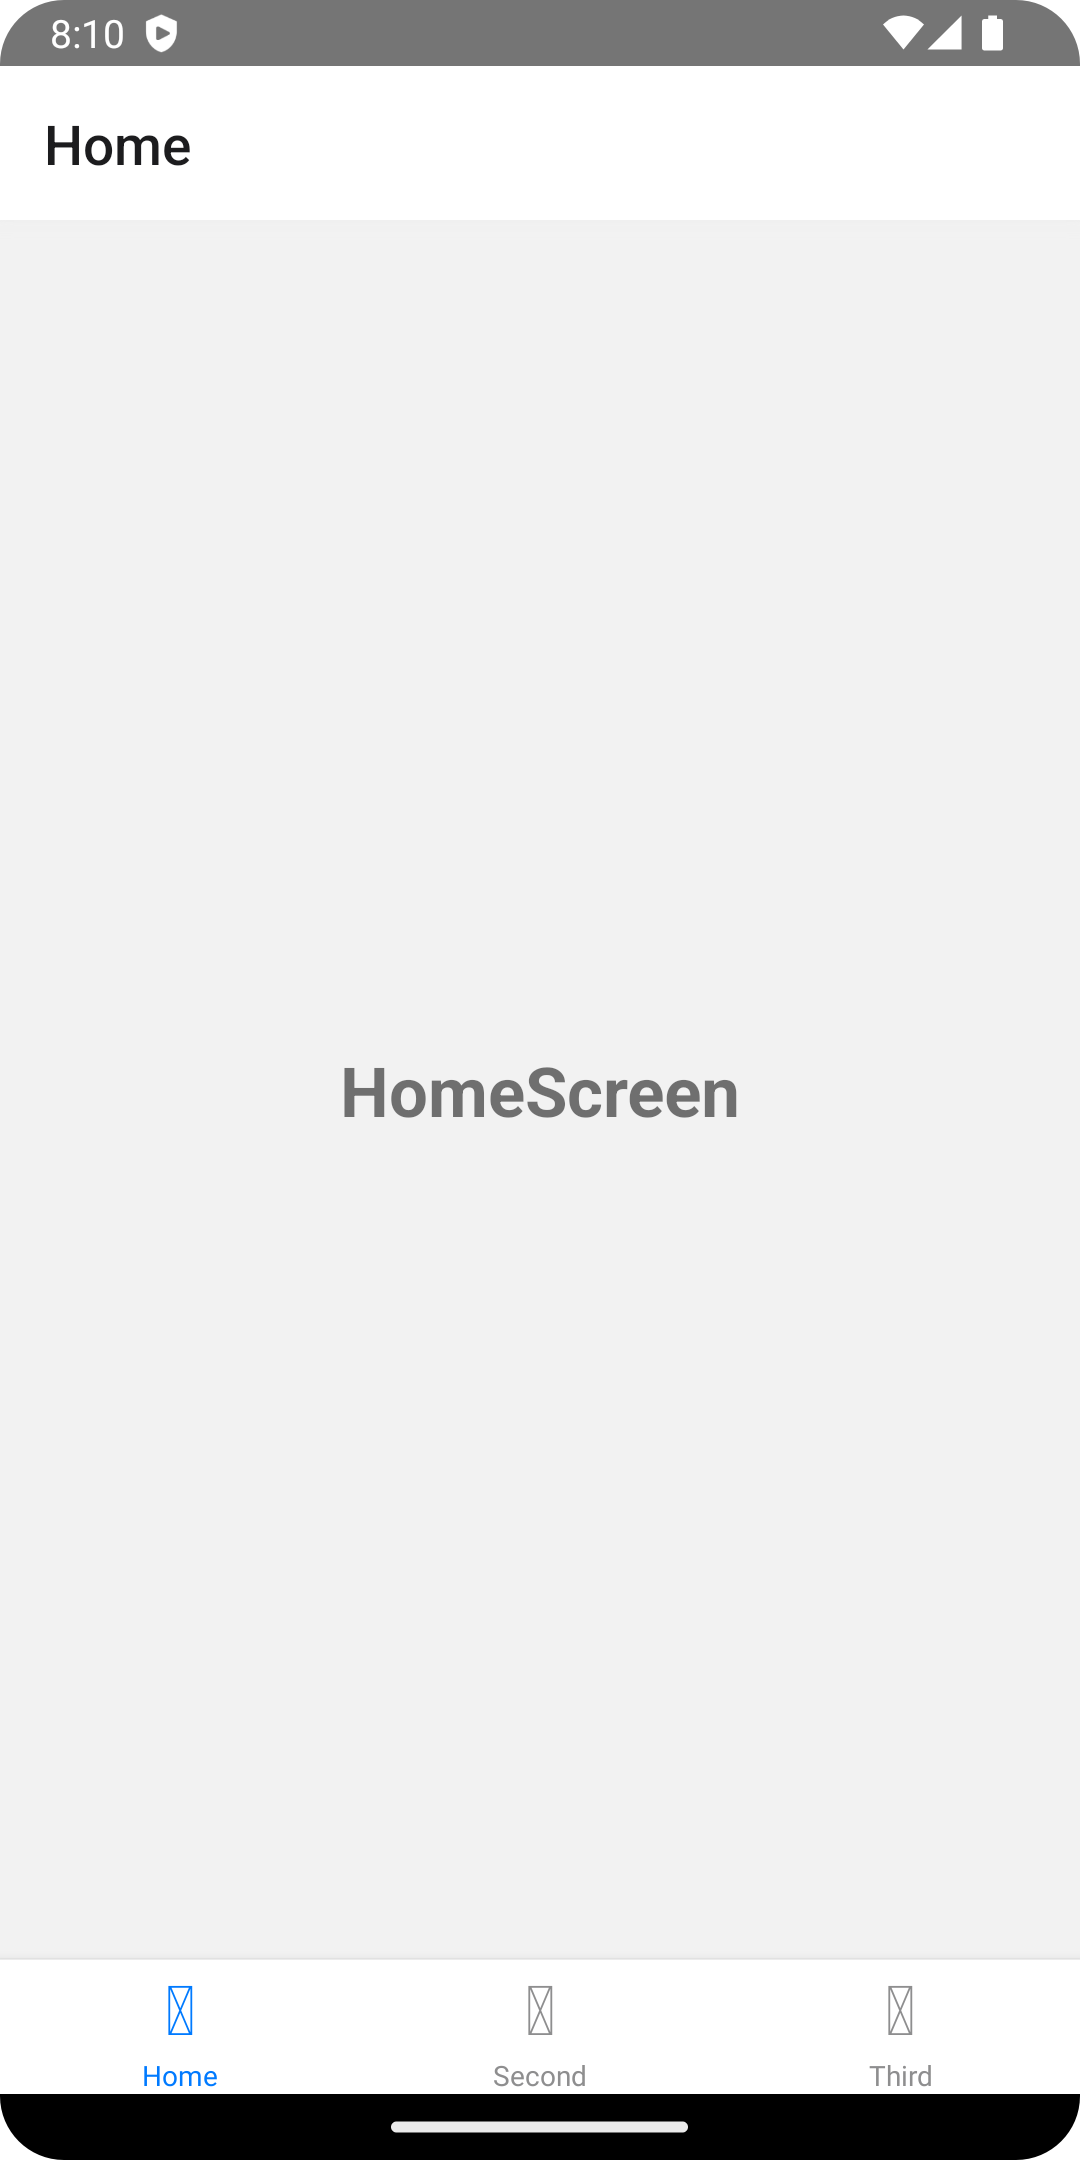
\includegraphics[height=0.4\textheight]{basis_layoutcross.png}
    \caption{Layout van applicatie voor de basisfunctionaliteiten bij React Native.}
\end{figure}


\subsubsection{Ontwikkeltijd}





\subsubsection{Performantie}

\paragraph{Tijdsduur}
\begin{figure}[H]
    \centering
    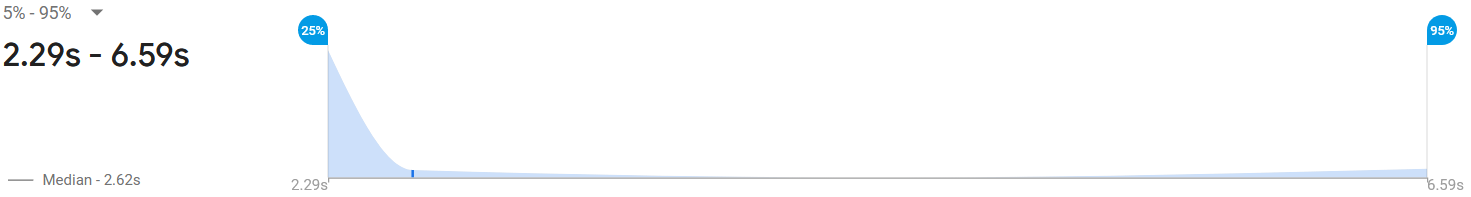
\includegraphics[height=0.1\textheight]{basisDuratieCross.png}
    \caption{Overzicht tijdsduur opstarten van applicatie met basisfunctionaliteiten bij React native.}
\end{figure}
Tijdens het meten van de duur voor het opstarten van de applicatie, 
is de applicatie meerdere keren opgestart. Op de grafiek is te zien dat de applicatie
gemiddeld 2,84 seconden nodig heeft om op te starten. Het minimum en maximum
liggen op 2,29 en 6,59 seconden.

\paragraph{CPU \& geheugen}
\begin{figure}[H]
    \centering
    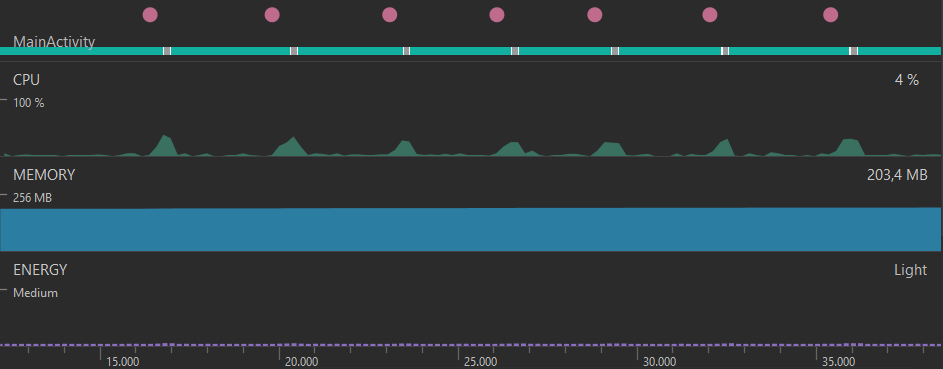
\includegraphics[height=0.25\textheight]{basisPerformantieCross.png}
    \caption{Overzicht CPU en geheugen gebruik tijdens het navigeren tussen schermen bij React native.}
\end{figure}
Net zoals bij native is op de grafiek te zien dat het CPU gebruik van de applicatie wanneer deze
inactief is, rond de 4\% ligt. En dat er duidelijk zichtbaar is wanneer er
genavigeerd wordt tussen de schermen. De piek van het CPU gebruik lag gemiddeld
op 32\% met een minimum en maximum van 27\% en 40\%. Wat bij React native opvalt is dat
het eerste keer navigeren naar een scherm een grotere piek geeft. Eenmaal dat het scherm 
al werd ingeladen is de piek minder groot. Dit wijst erop dat React native gebruik maakt van
lazy loading. Het geheugen blijft in tegenstelling
met de CPU wanneer de applicatie inactief en actief is, rond de 202MB hangen, met
verschillen van maximum 4-5MB. Er is geen merkbaar verschil in het geheugen wanneer
er genavigeerd wordt tussen de schermen.


\subsubsection{Schaalbaarheid}

\paragraph{Complexiteit}
Het gebruik van de libraries is niet complex. De navigatie is snel om op te zetten dankzij de documentatie van de library.
Het laadscherm is ook niet complex om op te zetten. Het enige dat nodig is, is een icon dat getoond zal worden en de 
initiële setup van de library. 

\paragraph{Herbruikbaarheid}
Het toevoegen van extra schermen is niet complex en kan dus makkelijk hergebruikt worden. Het is ook makkelijk om de
bestaande schermen te herbruiken in andere applicaties. Bij het laadscherm is er geen sprake van opschaling. Dit is enkel
nodig bij het opstarten van de applicatie en zal dus maar 1 keer geïmplementeerd moeten worden.



\section{Conclusie}






















